\documentclass{article}
    % General document formatting
    \usepackage[margin=0.7in]{geometry}
    \usepackage[parfill]{parskip}
    \usepackage[utf8]{inputenc}
    \usepackage{graphicx}
    \usepackage{fancyhdr}

    % Related to math
    \usepackage{amsmath,amssymb,amsfonts,amsthm}

    % Page Style
    \pagestyle{fancy}
    \fancyhf{}
    \rhead{Johannes Stricker}
    \lhead{Artificial Intelligence: Create A Domain-Independent Planner - Heuristic Analysis}
    \cfoot{\thepage}

\begin{document}

\section*{Non-Heuristic Search Analysis}
Three non-heuristic searches have been compared: Breadth First Search, Depth First
Search and Uniform Cost Search. From these three only Breadth First Search and Uniform
Cost Search were able to find optimal solutions for all three problems. Depth
First Search resulted in longer plans than necessary, which was to be expected given
the nature of how the search algorithm works. Because it searches depth first and returns
the first solution found, it will usually be a solution that includes many unnecessary
steps. The benefit of Depth First Search
was instead how quickly it found a solution, which became especially evident for problems
two and three, where it was on average 50 times faster than the other two non-heuristic
searches. \\
For the given problems it makes sense to spend a little more time on planning,
because making unnecessary plane flights would be more costly. Therefore one should choose
Breadth First Search or Uniform Cost Search if one has to choose from a non-heuristic
search method. However given a planning problem for which a few unnecessary steps are
cheap and planning time is crucial one might consider using Depth First Search instead.

\section*{Heuristic Search Analysis}
Both heuristic searches were able to find optimal solutions to all problems. A-Star
Search with the 'Ignore Preconditions' heuristic was almost 20 times faster on average
than with the 'Levelsum' heuristic, even though the latter expanded less nodes and
performed fewer goal tests. The reason for this is that the construction of the planning
graph that is required for the 'Levelsum' heuristic is very time consuming. Precisely
it requires $O(n(a+l)^2)$ operations, where $n$ is the number of levels the graph has,
$a$ ist the number of actions and $l$ is the number of literals. \cite{AIMA}\\
Compared to the non-heuristic searches, 'Ignore Preconditions' was slower only compared
to Depth First Search. For problem 1 Breadth First and Uniform Cost Search required
similar time, but for the other two problems they were outperformed. The explanation
for this is that when the search space is small, using good heuristics is less important, because
all solutions can be explored time-efficiently anyway and calculating complicated heuristics
might be even more time consuming. \\
The 'Levelsum' heuristic was slower than all of the non-heuristic searches for all
of the problems. It might become more effective when the search space grows even larger. \\
Therefore 'Ignore Preconditions' should be the preferred heuristic for planning
problems of this kind and it should be favored over non-heuristic strategies for
all non-trivial problems.

\section*{Results}
The results of solving the three air cargo problems using Breadth First Search,
Depth First Search, Uniform Cost Search and A-Star Search with the 'Ignore Preconditions'
and 'Levelsum' heuristics follow. \\
For each problem one optimal solution is provided. Please note that there is more than
one optimal solution to each of the problems.
\newpage

\subsection*{Problem 1}
$
Load(C1, P1, SFO) \rightarrow Fly(P1, SFO, JFK) \rightarrow Load(C2, P2, JFK)
\rightarrow Fly(P2, JFK, SFO) \rightarrow Unload(C1, P1, JFK) \rightarrow Unload(C2, P2, SFO)
$ \\
\begin{center}
  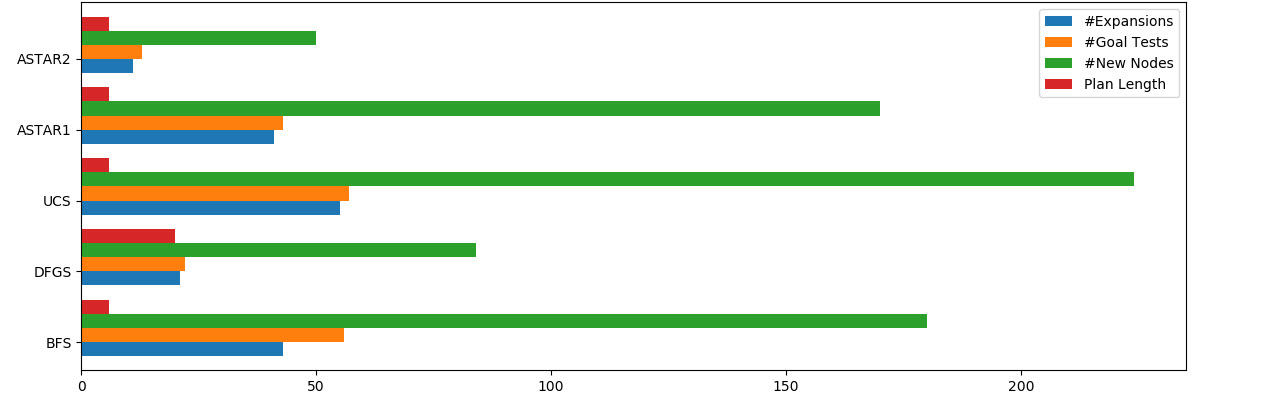
\includegraphics[width=\textwidth]{problem1.jpg}

  \begin{tabular}{ | l | l | l | l | l | l | }
    \hline
                                & #Expansions & #Goal Tests & #New Nodes  & Plan Length & Time Elapsed (sec) \\ \hline \hline
    Breadth First Search        & 43          & 56          & 180         & 6   & 0.04  \\ \hline
    Depth First Search          & 21          & 22          & 84          & 20  & 0.01  \\ \hline
    Uniform Cost Search         & 55          & 57          & 224         & 6   & 0.03  \\ \hline
    A* [Ignore Preconditions]   & 41          & 43          & 170         & 6   & 0.04  \\ \hline
    A* [Levelsum]               & 11          & 13          & 50          & 6   & 0.77  \\ \hline
  \end{tabular}
\end{center} \\ \\

\subsection*{Problem 2}
$
Load(C1, P1, SFO) \rightarrow Fly(P1, SFO, JFK) \rightarrow Load(C2, P2, JFK)
\rightarrow Fly(P2, JFK, SFO) \rightarrow Load(C3, P3, ATL) \rightarrow Fly(P3, ATL, SFO)
\rightarrow Unload(C3, P3, SFO) \rightarrow Unload(C2, P2, SFO) \rightarrow Unload(C1, P1, JFK)
$ \\ \\

\begin{center}
  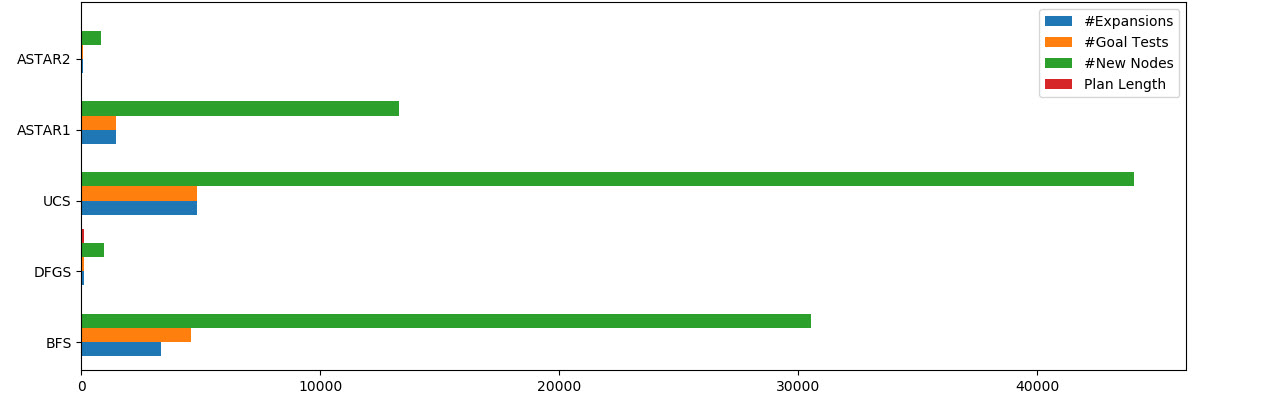
\includegraphics[width=\textwidth]{problem2.jpg}

  \begin{tabular}{ | l | l | l | l | l | l | }
    \hline
                                & #Expansions & #Goal Tests & #New Nodes  & Plan Length & Time Elapsed (sec) \\ \hline \hline
    Breadth First Search        & 3346        & 4612        & 30534       & 9     & 13.50 \\ \hline
    Depth First Search          & 107         & 108         & 959         & 105   & 0.32  \\ \hline
    Uniform Cost Search         & 4853        & 4855        & 44041       & 9     & 11.91 \\ \hline
    A* [Ignore Preconditions]   & 1450        & 1452        & 13303       & 9     & 4.29  \\ \hline
    A* [Levelsum]               & 86          & 88          & 841         & 9     & 68.31 \\ \hline
  \end{tabular}
\end{center} \\ \\

\subsection*{Problem 3}
$
Load(C2, P2, JFK) \rightarrow Fly(P2, JFK, ORD) \rightarrow Load(C4, P2, ORD)
\rightarrow Fly(P2, ORD, SFO) \rightarrow Load(C1, P1, SFO) \rightarrow Fly(P1, SFO, ATL)
\rightarrow Load(C3, P1, ATL) \rightarrow Fly(P1, ATL, JFK) \rightarrow Unload(C4, P2, SFO)
\rightarrow Unload(C3, P1, JFK) \rightarrow Unload(C2, P2, SFO) \rightarrow Unload(C1, P1, JFK)
$ \\

\begin{center}
  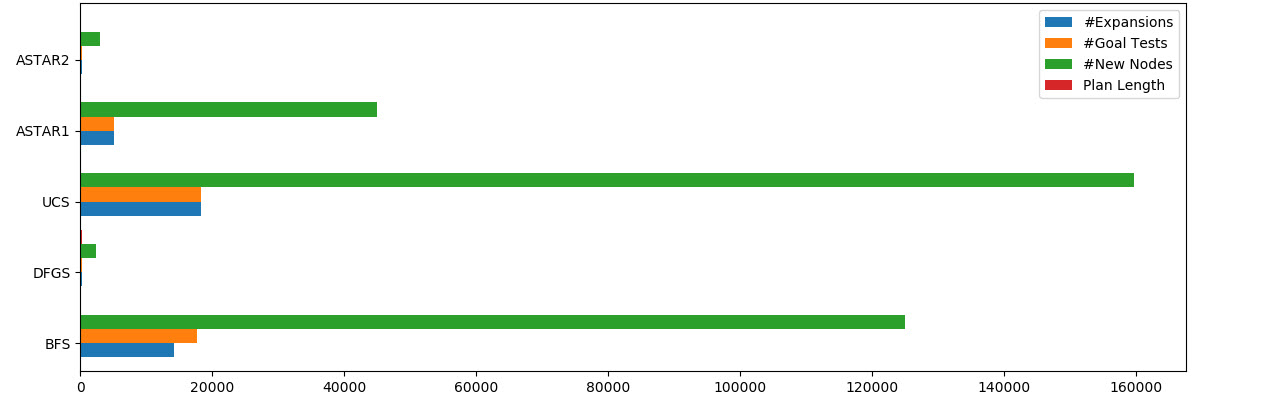
\includegraphics[width=\textwidth]{problem3.jpg}

  \begin{tabular}{ | l | l | l | l | l | l | }
    \hline
                                & #Expansions & #Goal Tests & #New Nodes  & Plan Length & Time Elapsed (sec) \\ \hline \hline
    Breadth First Search        & 14120       & 17673       & 124926      & 12    & 98.33   \\ \hline
    Depth First Search          & 292         & 293         & 2388        & 288   & 1.16    \\ \hline
    Uniform Cost Search         & 18223       & 18225       & 159618      & 12    & 55.00   \\ \hline
    A* [Ignore Preconditions]   & 5040        & 5042        & 44944       & 12    & 17.70   \\ \hline
    A* [Levelsum]               & 315         & 317         & 2902        & 12    & 358.67  \\ \hline
  \end{tabular}
\end{center} \\ \\

\begin{thebibliography}{1}
\bibitem[Russel and Norvig (2010)]{AIMA} Stuart Russel and Peter Norvig {\em Artificial Intelligence - A Modern
Approach 3rd Edition} 2010.
\end{thebibliography}
\end{document}
